\chapter{Evaluation}

This chapter covers the evaluation of this active object system. The evaluation is split into three parts. The first part covers the basic functionality, where the quality of the sensor data, the results of the computer vision, problems with the navigation and the general system stability are discussed. In the second part the quality of the generated maps is investigated. The last part evaluates the search performance, both within single rooms and in larger indoor environments.

Three environments were available for testing. Environment 1 is a home environment in a small flat, consisting of three rooms. Environment 2 is an atypical university environment consisting of some offices and the robotics-lab. Environment 3 is a part of an university floor with rooms of various types. A more detailed description of the environments can be found in section \ref{EvalMapping}.

\section{Basic Functionality}

This section is no detailed evaluation of the basic functionality of the robot system, but only an overview for better understanding of the results in the following sections.

\subsection{Sensor Data}

\subsubsection{Laser scans}

The accuracy of the range measurements from the LIDAR were found to be accurate enough for the creation of good quality maps. However, the limited range of the sensor, which is only 4\,m, causes problems in open areas and corridors. Firstly, without valid range measurements the localization of the robot has to rely on the odometry, which can lead to inaccurate results. Secondly, some obstacles are not detected. Obviously, the LIDAR has problems with glass and reflecting surfaces, but also some other surfaces are not reliably detected. The combination of those two problems is difficult to handle, as described in section \ref{preprocessing}, and has therefore a negative impact on the map quality.

\subsubsection{RGB-images}

The low resolution of the images is no problem because the CNNs do not use higher resolutions anyway. More problematic is the mediocre quality of the images. The CNNs can handle the noise pretty well, but the low dynamic range prevents the object detection from detecting objects in bad lit areas and the necessary high exposure time leads to motion blur. This is especially noticeable when the robot rotates. Therefore the rotational velocity during exploration and search is limited and generally images are discarded if the robot rotates too fast. In figure \ref{RotMax} an image taken with the maximum allowed rotation is shown. Small, distant objects are not detected reliably anymore. However, decreasing the maximum rotational velocity would result in very slow object searches.

\begin{figure}[h]
\centering
  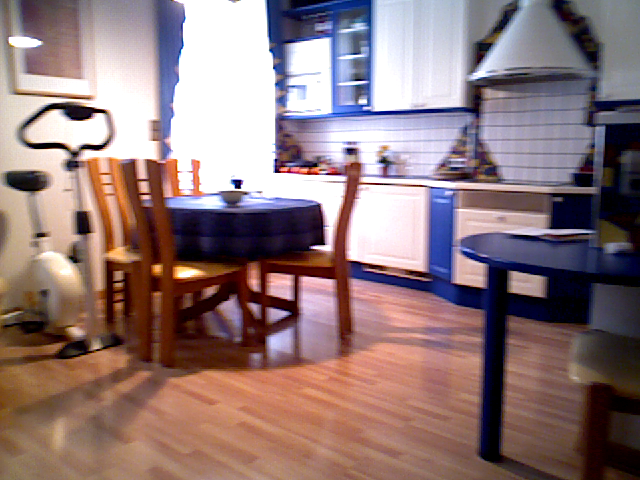
\includegraphics[width=0.7\textwidth,clip]{figures/basic_eval/max_rot_img.png} 
  \caption[Example RGB-image]{An example RGB-image: At the maximum rotational velocity the motion blur is already high. The limited dynamic range is also visible in this image. }
  \label{RotMax}
\end{figure}

\subsubsection{Point clouds}

The quality of the point cloud is good, but obviously not as accurate as the laser scan. The distance range given in the specifications of the RGBD-camera from 0.8\,m to 3.5\,m is very pessimistic. Tests showed a minimum detectable distance of 0.55\,m and a maximum distance much higher than the 3.5\,m. 

\subsection{Computer vision}

\subsubsection{Room type classification}



\subsubsection{Object detection}

\subsubsection{Doorway detection}

The doorway detection works very well, with no wrong detections and no passing of undetected doorways during the test runs. The only problem is the small field of view of the upward looking RGBD-camera. Therefore doorways are only detected if the robot is near the doorway and facing towards the doorway. This means that a doorway may not be detected while driving by.

\subsection{Navigation}

The navigation causes a lot of problems in this work. The main problem is the high payload, which puts too much weight on the passive wheels. This results in less grip on the active wheels. As a result the robot has problems to turn, especially on slippery or uneven ground. In some cases the robot is even unable to turn at all without some help. When executing in-place rotations the robot might drift forwards or backwards. The biggest problem is that the robot has problems to drive curves as planned. The slipping caused the robot to drive curves too wide, which in further consequence lead the robot to get stuck because it got too near to an obstacle. The recovery behaviors may be successful, but sometimes the robot needs help to unstuck. This problem was somewhat solved by increasing all rotational velocities manually before sending them to the Turtlebot. 

\subsection{System Stability}

\section{Mapping}

The quality of the maps are investigated after a complete exploration of the environment without object search. This was done in all three environments multiple times. In this section typical results of those exploration runs are presented and also encountered problems. At first the metric maps are investigated, followed by the Room-Type-Maps and the Object-Maps. At the end of this section the resulting Object-Probability-Maps and the total object probabilities are discussed.

\subsection{Hybrid Metric Map} \label{EvalMapping}

In figure \ref{map2d_home}, figure \ref{map2d_lab} and figure \ref{map2d_ist} maps created in the three environments are shown. The 2D maps of the rooms have in general good quality, especially in the small rooms. All maps contain cells wrongly set to free outside of the room. On the one hand those are caused by reflexion and transparent surfaces. On the other hand they are caused by the handling of invalid range measurements described in section \ref{preprocessing}. However those cause no major problems. The maps of the rooms lab1 and institute1 are distorted. In the map of room lab1 the top part leans to the left while the bottom right part is rotated towards the bottom right part. In the map of room institute1 the bottom corridor is curved upwards. The distortion in both rooms are probably caused by a conjunction of inaccurate odometry and insufficient distinct features in the visible by the LIDAR. These distortion show the benefit of the hybrid map design. The maps are still sufficiently accurate, but those distortion become more and more problematic with larger maps. As can be seen in the maps the doorway poses are all quiet accurate. 

\begin{figure}
\centering
  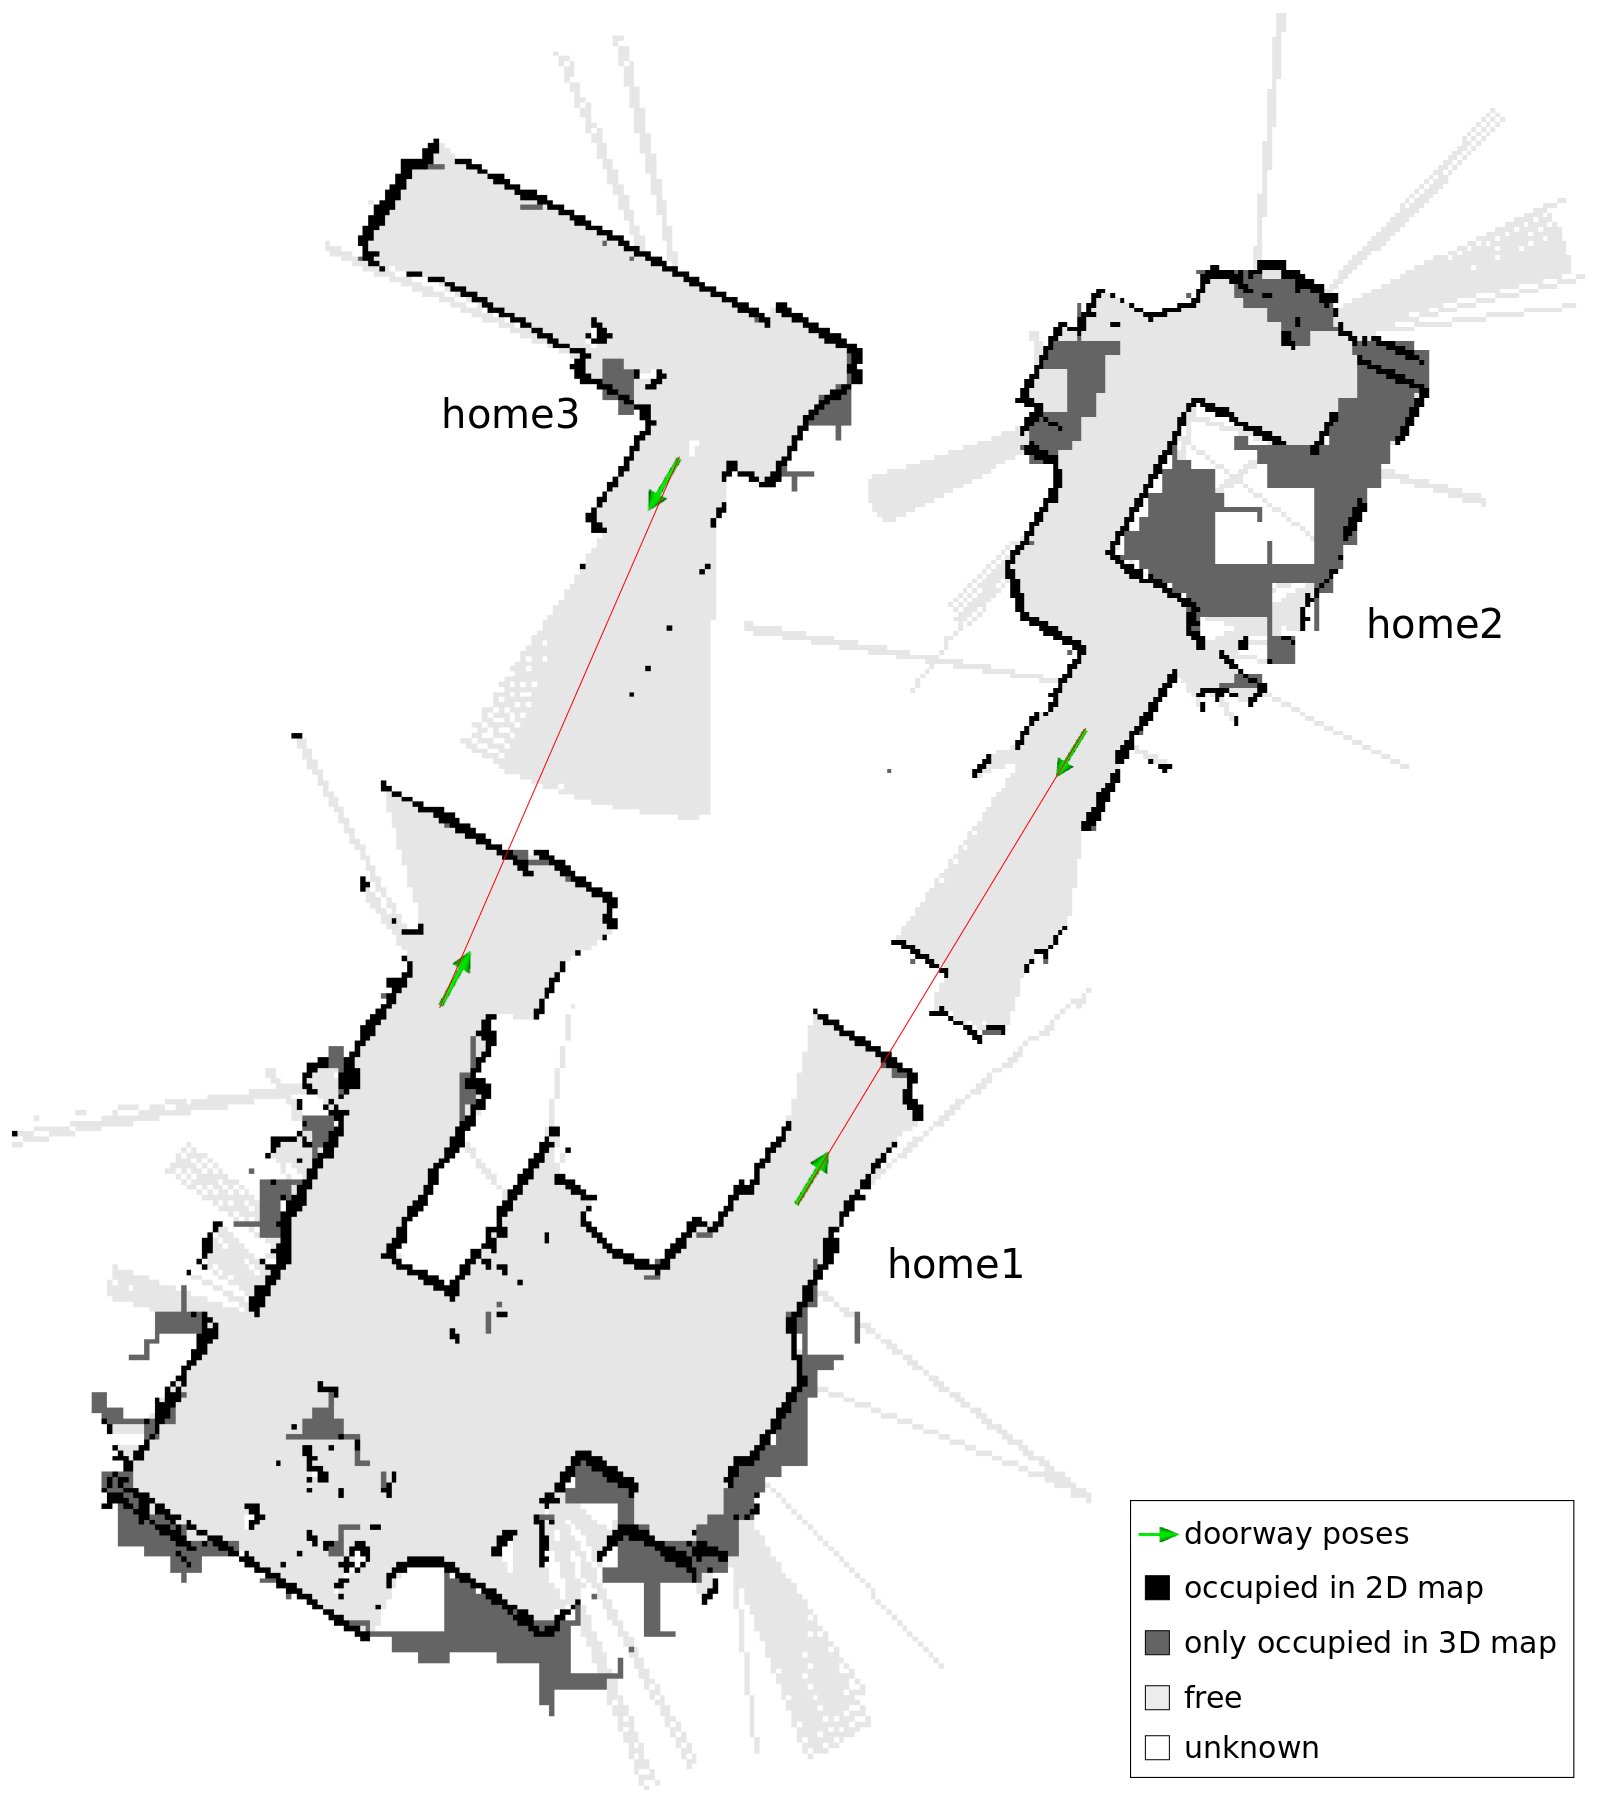
\includegraphics[width=0.9\textwidth,clip]{figures/2Dmaps/all5.png}
  \caption[Hybrid map of the home environment]{Hybrid map of the home environment: The room home1 is combination of a kitchen and a living room, the room home2 is a bedroom with an office-like area in the upper right corner and the room home3 is an anteroom.}
  \label{map2d_home}
\end{figure}

\begin{figure}
\centering
  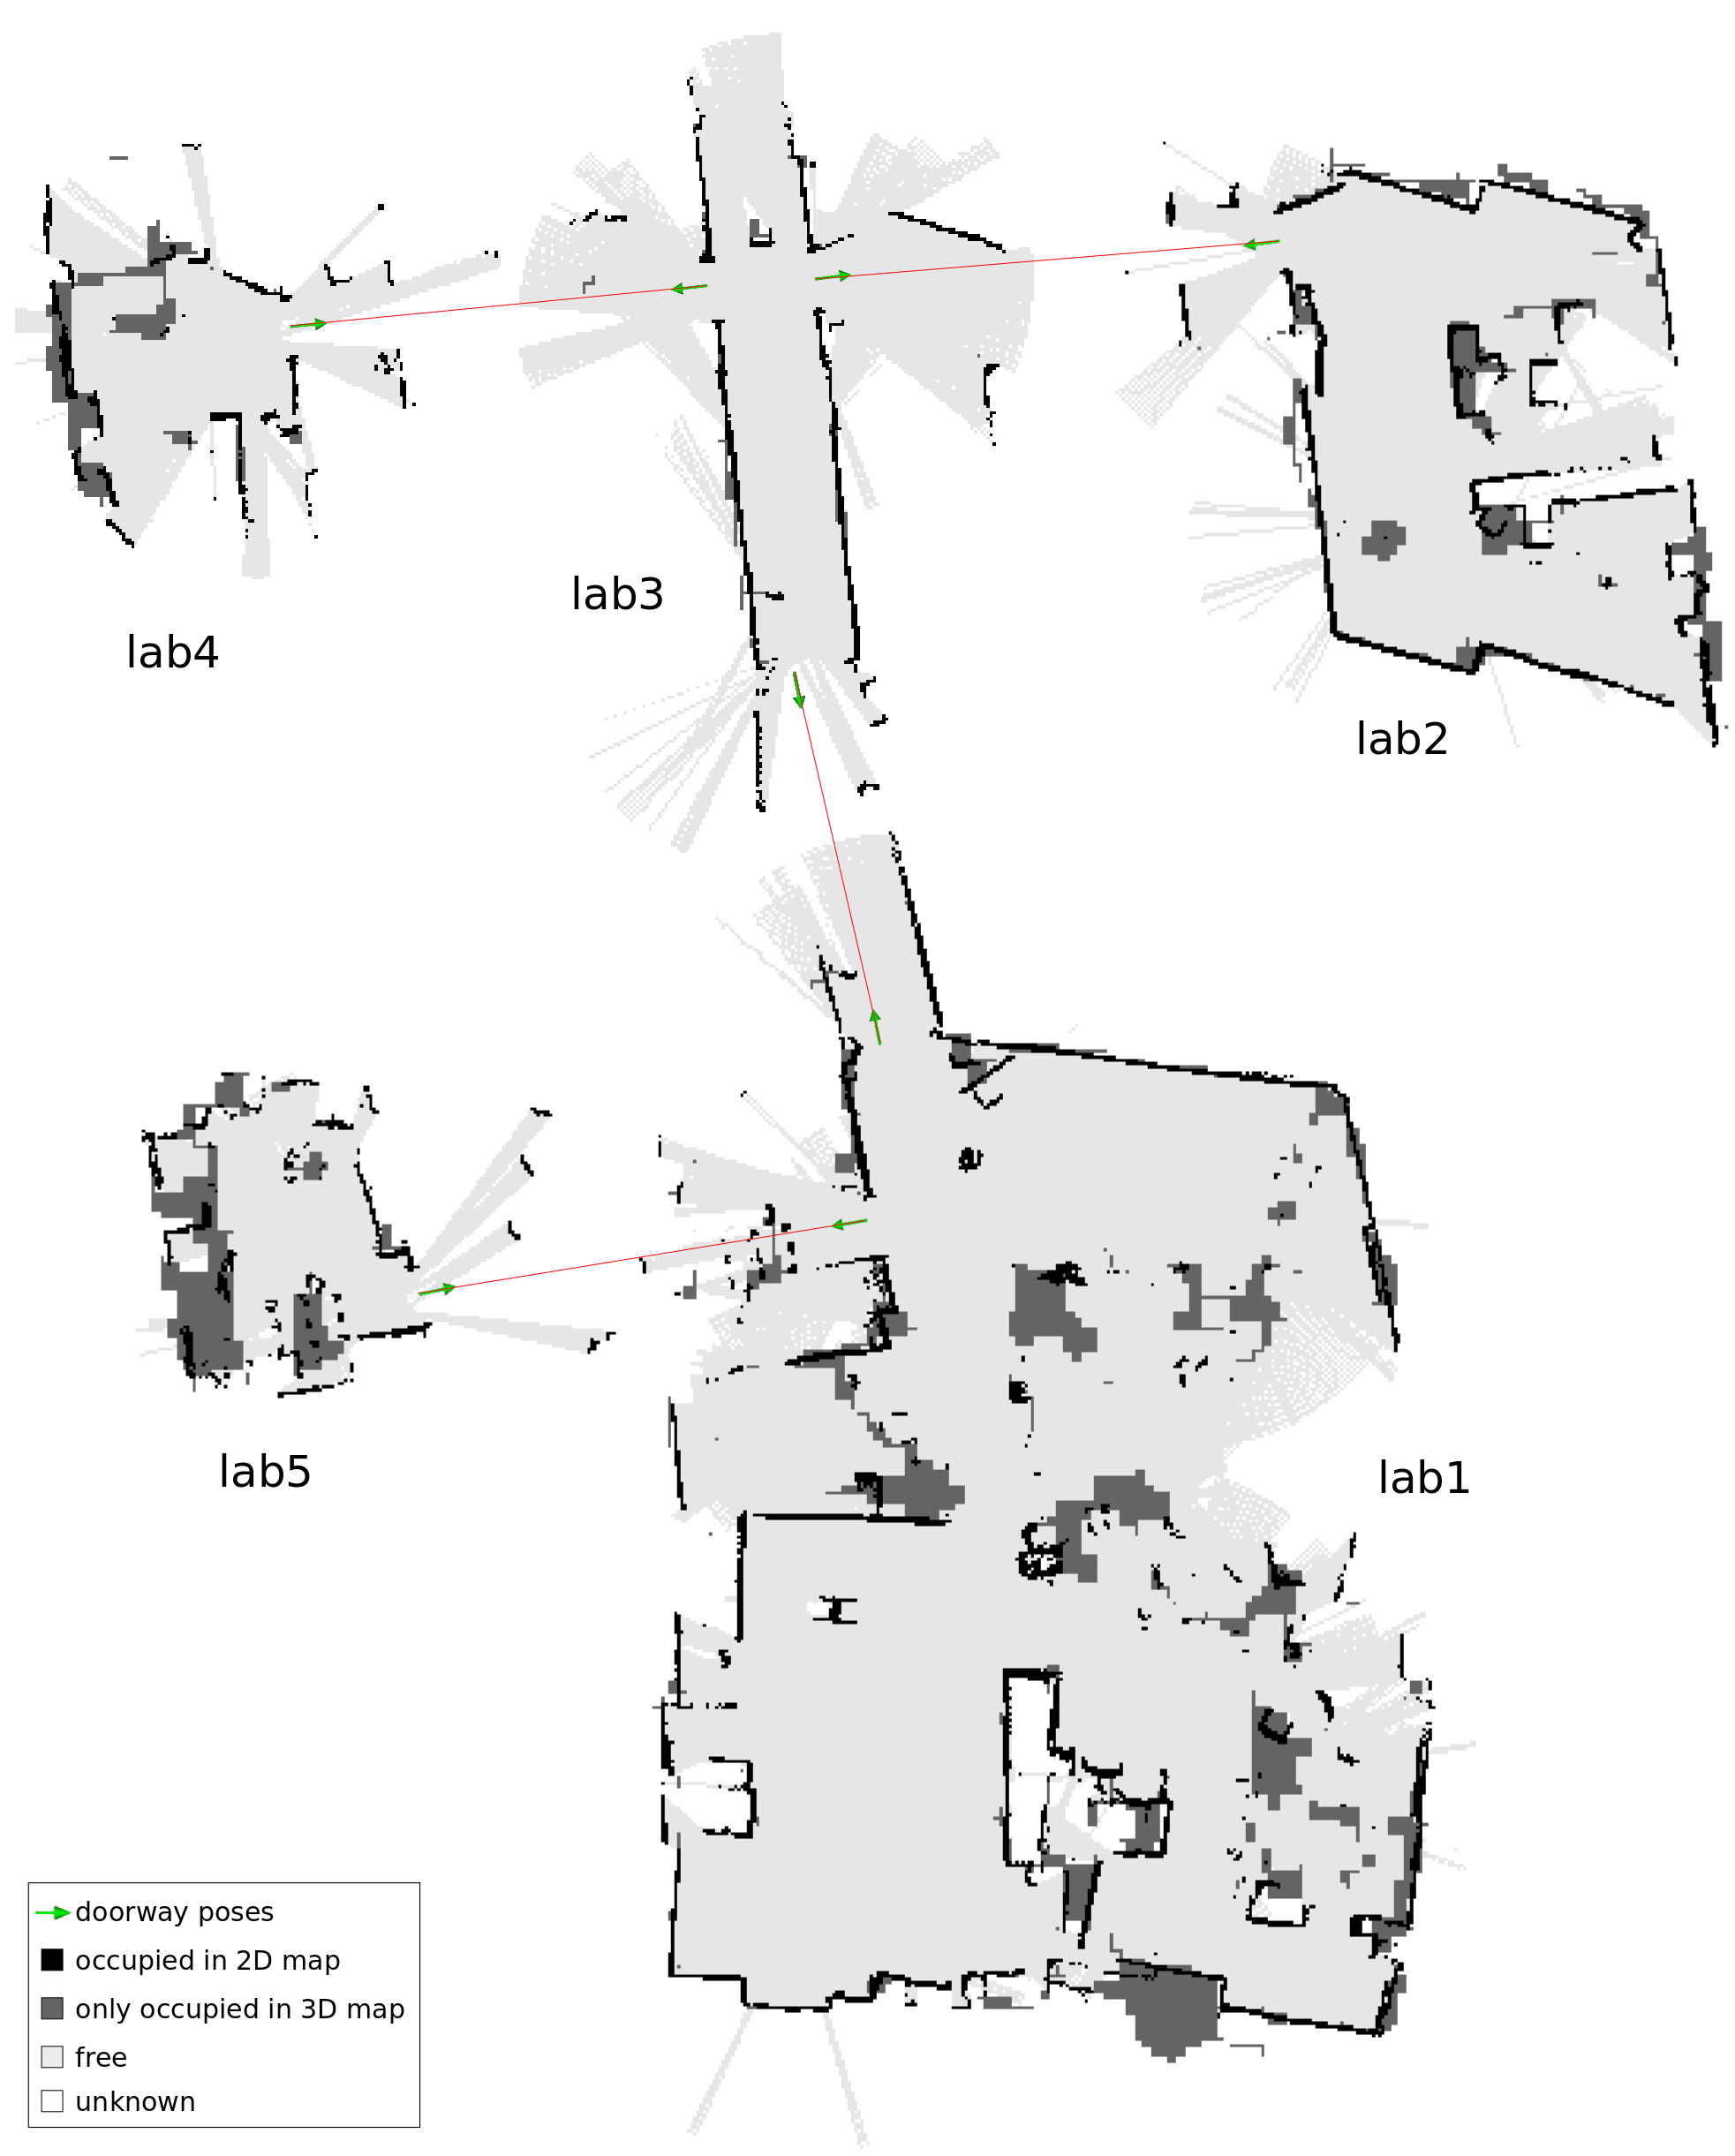
\includegraphics[width=0.99\textwidth,clip]{figures/2Dmaps/all_lab.png}
  \caption[Hybrid map of the robotics-lab environment]{Hybrid map of robotics-lab environment: The room lab1 is the robotics-lab, which consists mainly of an office area and has free space at the botton left and a sofa and a kitchen area at the bottom right. The room lab2 is an office, the room lab3 is a corridor, the room lab4 is also an office and the room lab5 is a workshop/storage room.}
  \label{map2d_lab}
\end{figure}

\begin{figure}
\centering
  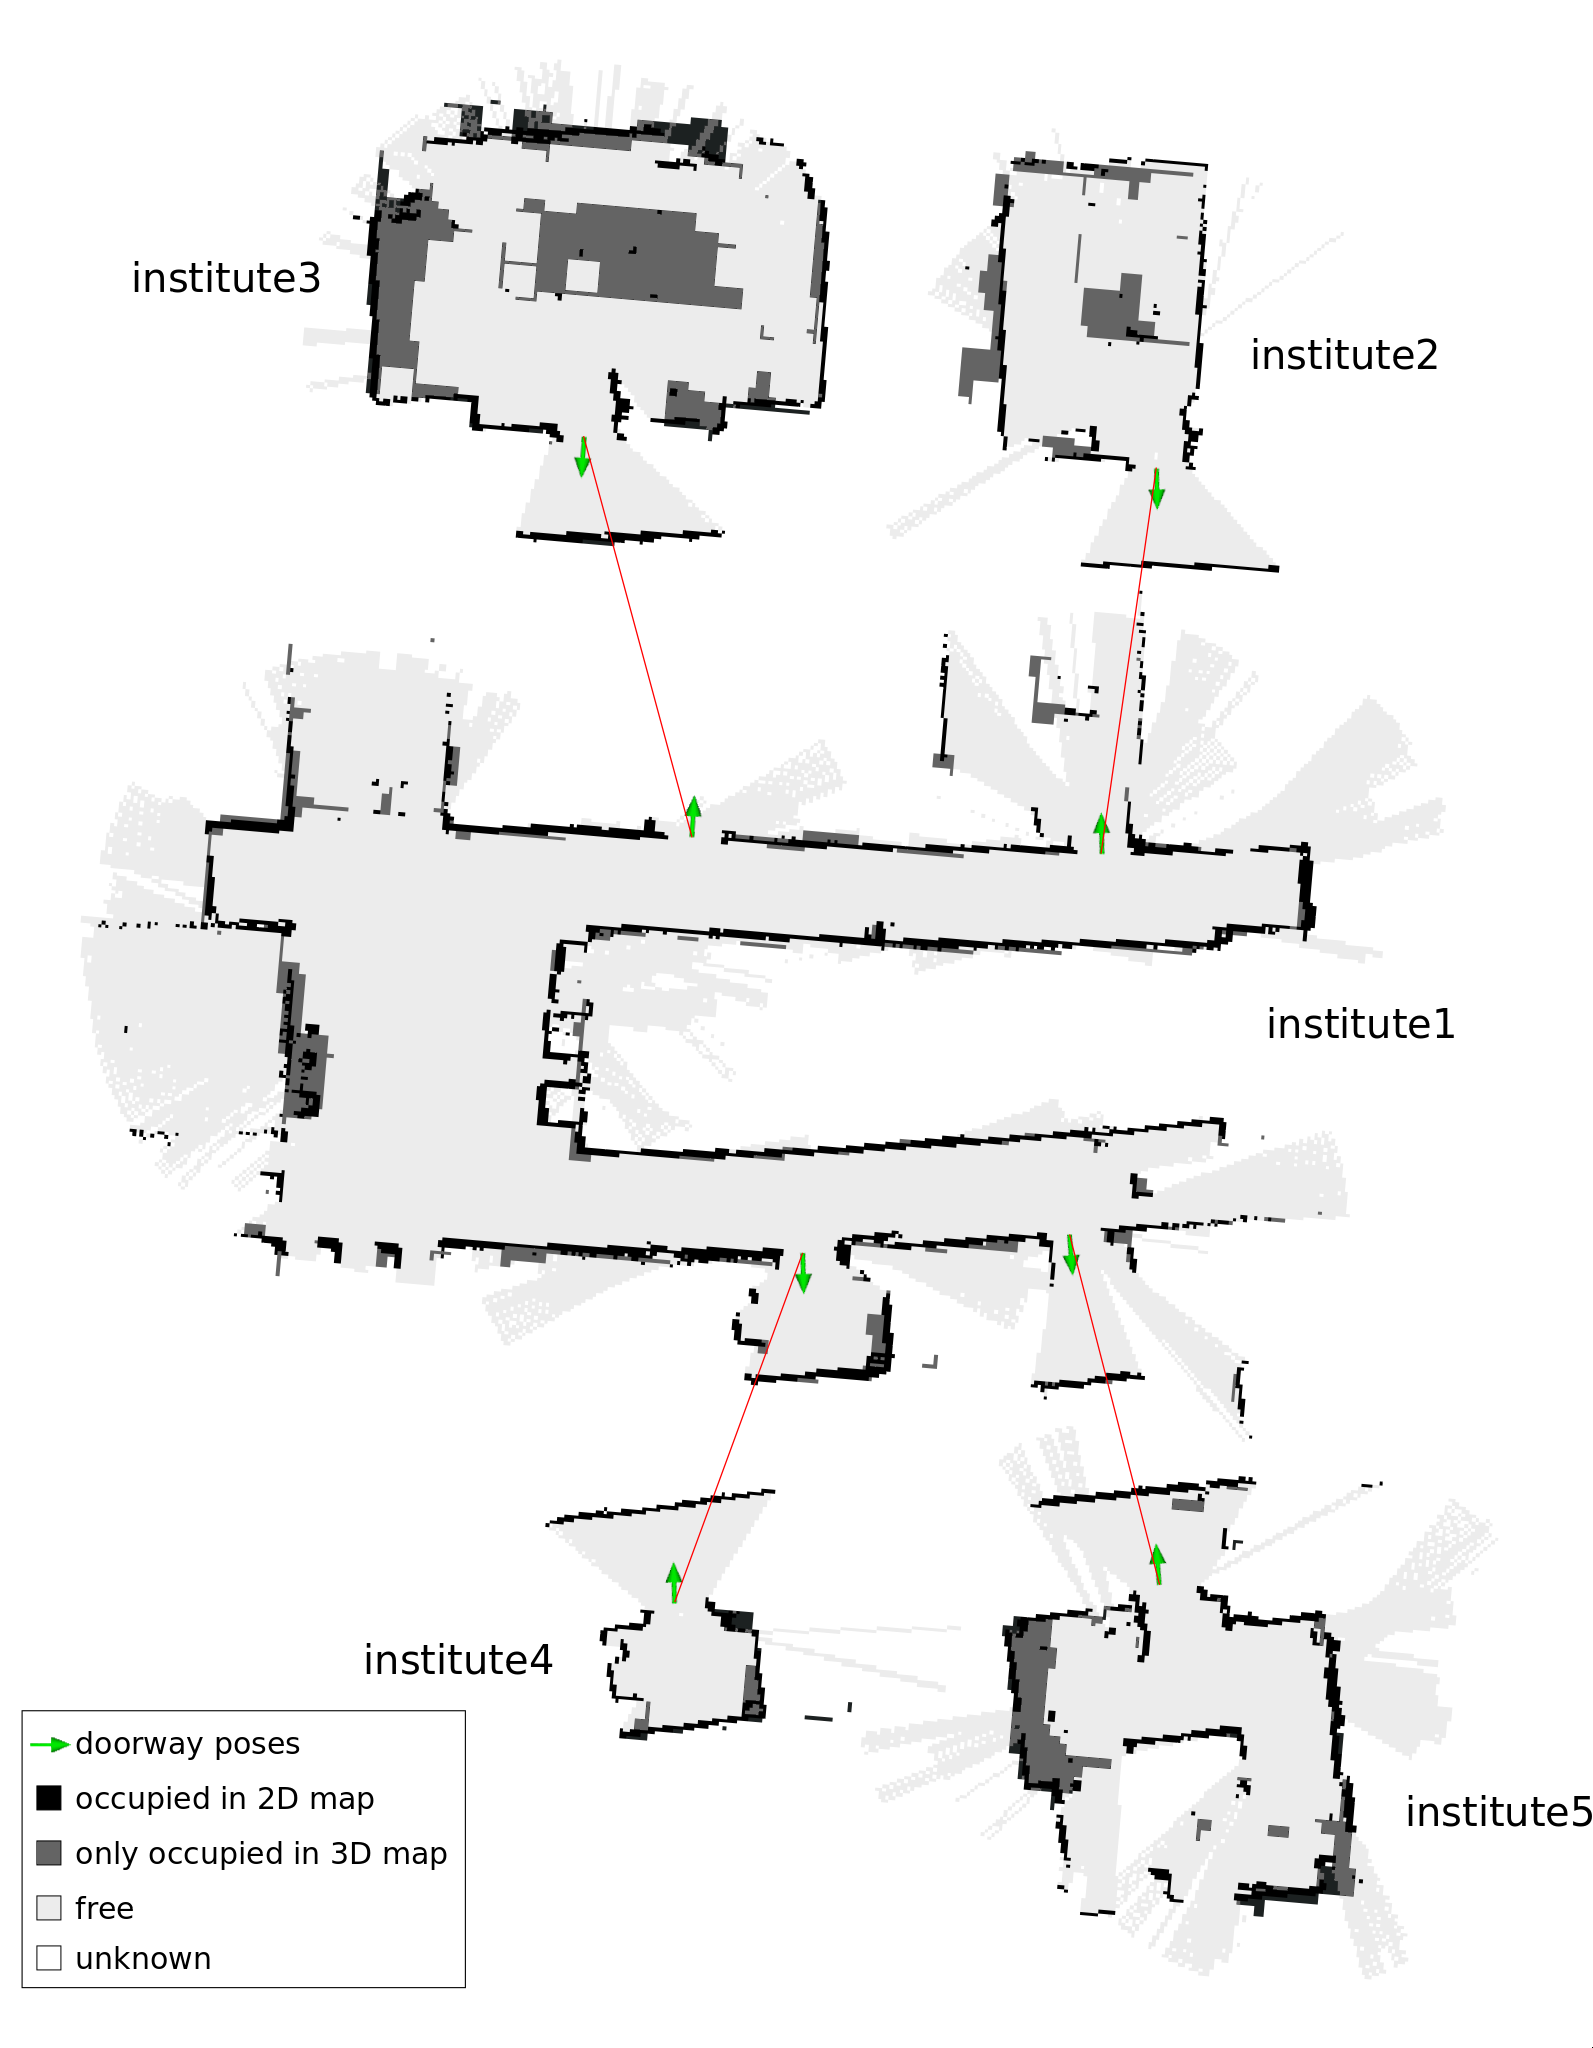
\includegraphics[width=0.9\textwidth,clip]{figures/2Dmaps/all_IST_b.png}
  \caption[Hybrid map of the university floor]{Hybrid map of a part of an university floor: The room institute1 is a corridor with an copy area, the room institute2 contains a kitchen area and a dining table, the room institute3 is a meeting room, the room institute4 is a bathroom and the room institute5 is a secretariat. }
  \label{map2d_ist}
\end{figure}

\subsection{Room Type Map}

\begin{figure}
\renewcommand*\thesubfigure{\arabic{subfigure}} 
\centering
\begin{tabular}{cc}
\subfloat[]{
\includegraphics[width=0.45\textwidth]{figures/wz_imgs/1.png}} &
\subfloat[]{
\includegraphics[width=0.45\textwidth]{figures/wz_imgs/2.png}} \\
\subfloat[]{
\includegraphics[width=0.45\textwidth]{figures/wz_imgs/3.png}} &
\subfloat[]{
\includegraphics[width=0.45\textwidth]{figures/wz_imgs/4.png}} \\
\subfloat[]{
\includegraphics[width=0.45\textwidth]{figures/wz_imgs/5.png}} &
\subfloat[]{
\includegraphics[width=0.45\textwidth]{figures/wz_imgs/6.png}}
\end{tabular}
\caption[Images of the room home1]{Images with place classification results of the room home1}
\label{wz_imgs}
\end{figure}

\begin{figure}
\centering
  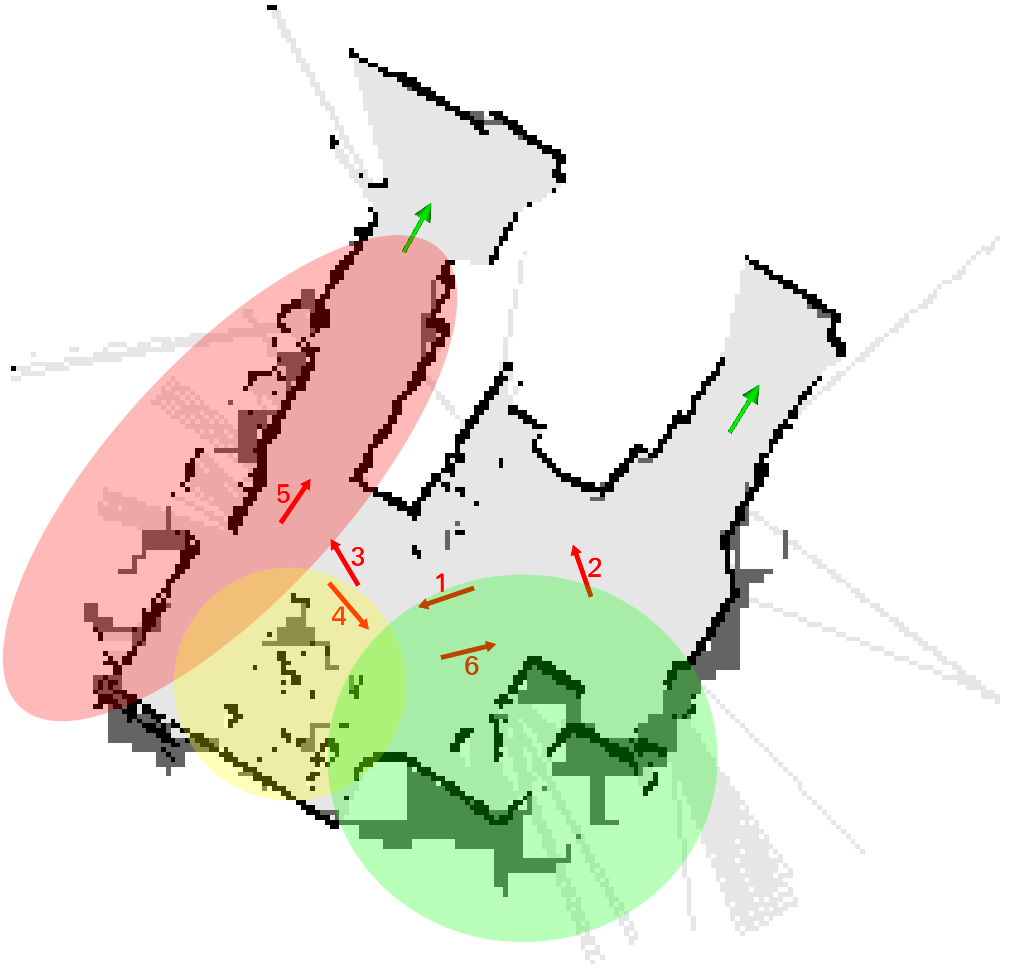
\includegraphics[width=0.9\textwidth, trim=0 0 50 0,clip]{figures/wz_imgs/wz_views_b.png}
  \caption[Detailed map of the room home1 with image poses]{Detailed map of the room home1: Green arrows mark the doorways, the numbered red arrows are the view poses of the corresponding images from figure \ref{wz_imgs}}.
  \label{wz_views}
\end{figure}

\begin{figure}
\centering
\begin{tabular}{ccc}
\subfloat[run 1]{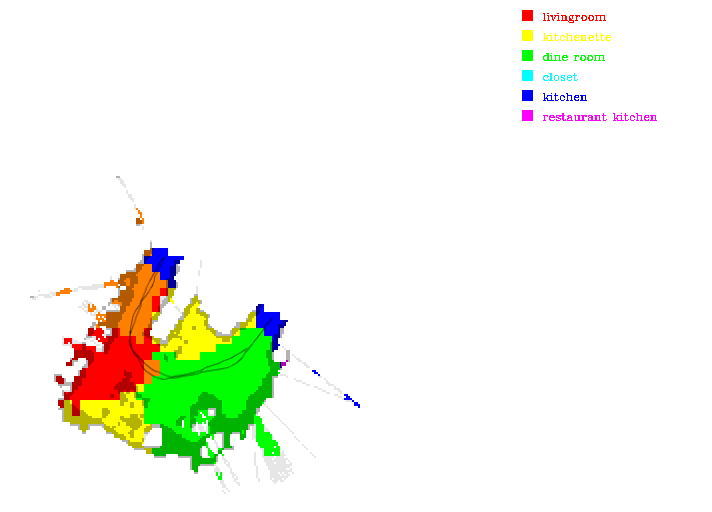
\includegraphics[width=0.3\textwidth,trim=40 10 360 250, clip]{figures/wz_imgs/h5e/classes_0_b.png}} &
\subfloat[run 1, without room type correlation]{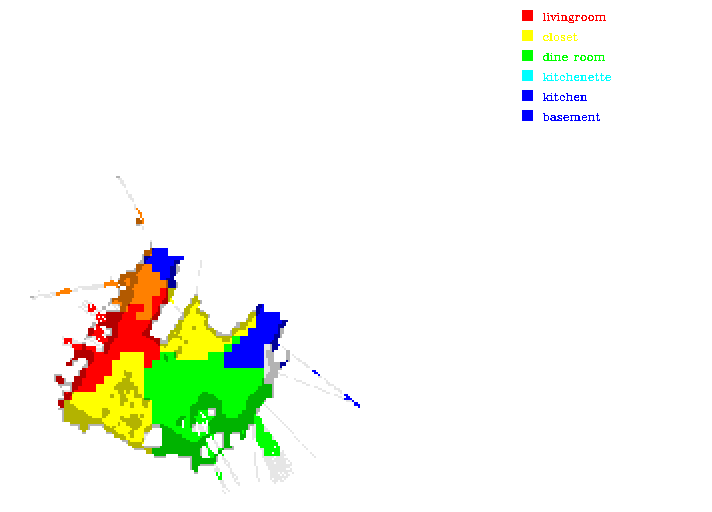
\includegraphics[width=0.3\textwidth,trim=40 10 360 250, clip]{figures/wz_imgs/h5e/classes_1_b.png}} &
\subfloat[run 2]{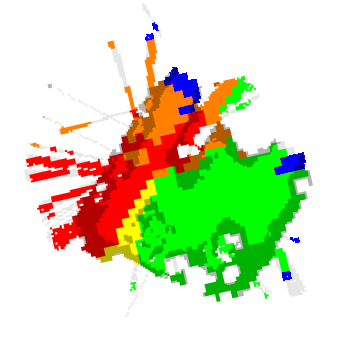
\includegraphics[width=0.3\textwidth,trim=0 20 0 50,clip]{figures/wz_imgs/h5e/classes_2_b_b2.png}} \\
\subfloat[run 3]{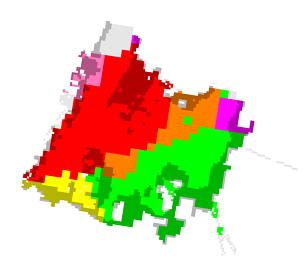
\includegraphics[width=0.3\textwidth,trim=30 0 0 50,clip]{figures/wz_imgs/h5e/classes_3_b.png}} &
\subfloat[after executed search]{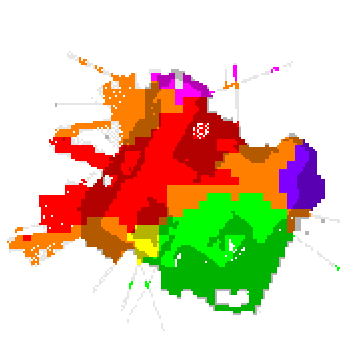
\includegraphics[width=0.3\textwidth,trim=0 0 0 50,clip]{figures/wz_imgs/h5e/classes_search_b.png}} &
\subfloat{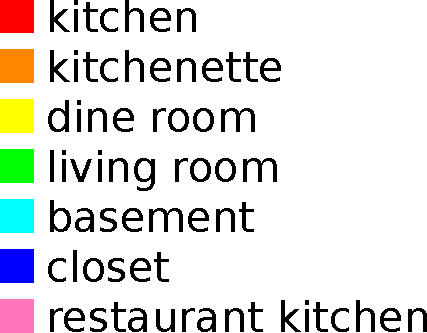
\includegraphics[width=0.3\textwidth,trim=-50 0 0 0, clip]{figures/wz_imgs/h5e/legend.pdf}} 
\end{tabular}
\caption[Map of most likely room types for the room home1]{Map of most likely room types for the room home1}
\label{frontier_calc}
\end{figure}

\begin{figure}
\centering
\begin{tabular}{ccc}
\subfloat[kitchen]{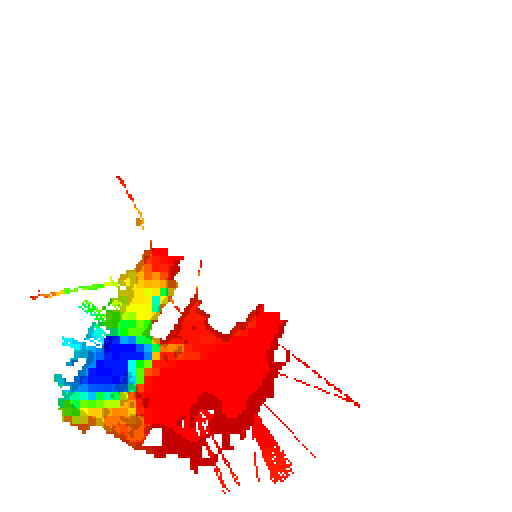
\includegraphics[width=0.3\textwidth,trim=40 10 160 250, clip]{figures/wz_imgs/h5e/kitchen_b.png}} & 
\subfloat[kitchenette]{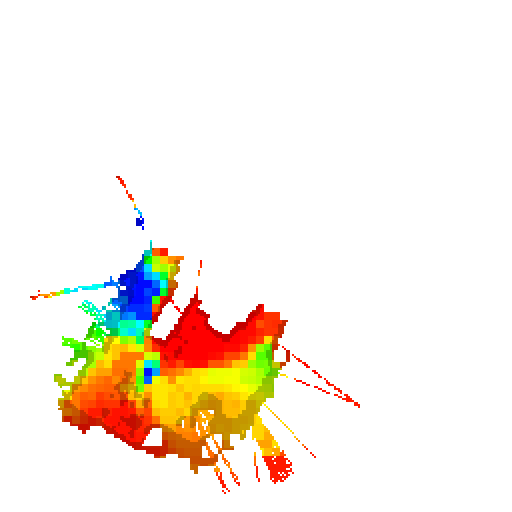
\includegraphics[width=0.3\textwidth,trim=40 10 160 250, clip]{figures/wz_imgs/h5e/kitchenette_b.png}} &
\subfloat[living room]{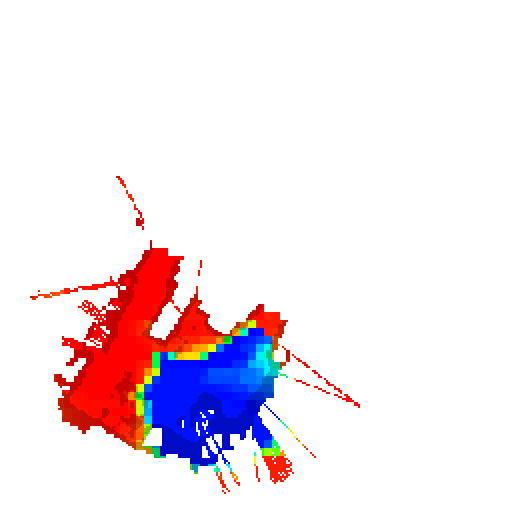
\includegraphics[width=0.3\textwidth,trim=40 10 160 250, clip]{figures/wz_imgs/h5e/livingroom_b.png}} \\
\subfloat[dine room]{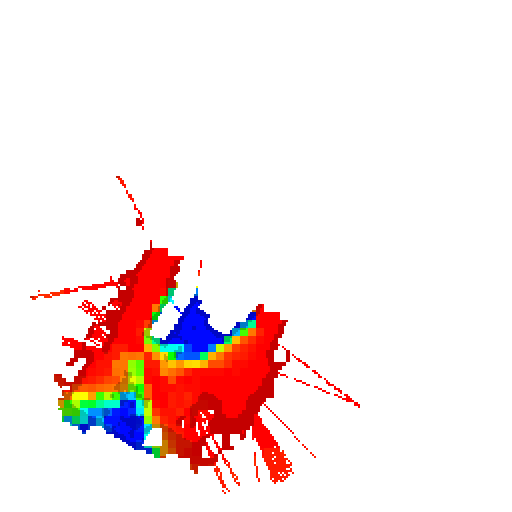
\includegraphics[width=0.3\textwidth,trim=40 10 160 250, clip]{figures/wz_imgs/h5e/dine_b.png}} &
\subfloat[closet]{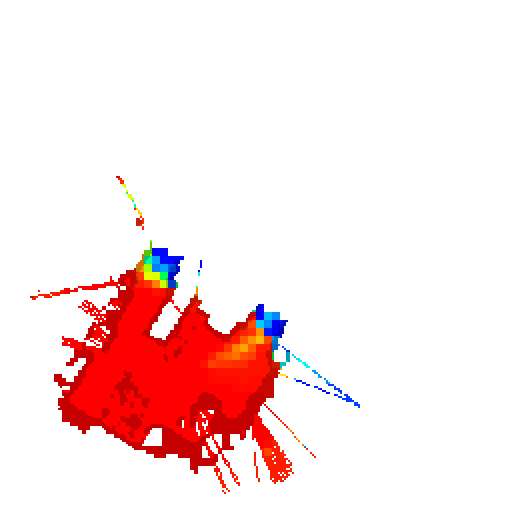
\includegraphics[width=0.3\textwidth,trim=40 10 160 250, clip]{figures/wz_imgs/h5e/closet_b.png}} &
\subfloat{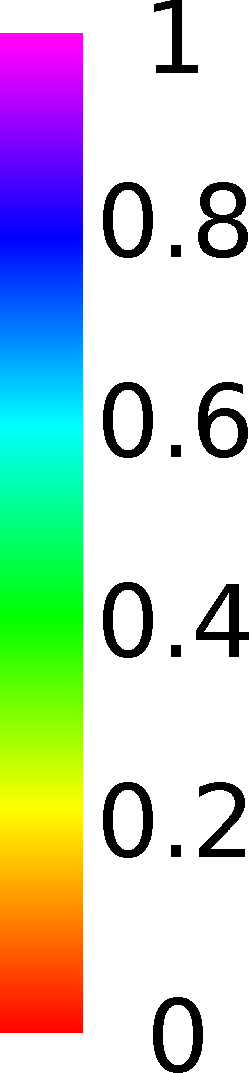
\includegraphics[width=0.3\textwidth,trim=-300 0 -300 0, clip]{figures/wz_imgs/h5e/problegend.pdf}} 
\end{tabular}
\caption{Probabilities of stated room type in room home 1}
\label{frontier_calc}
\end{figure}

\subsection{Object Map}



\subsection{Information after Peek Task}

\begin{figure}
\centering
\begin{tabular}{ccc}
\subfloat[office: 0.4442 \newline home office: 0.3214 \newline attic: 0.0174]{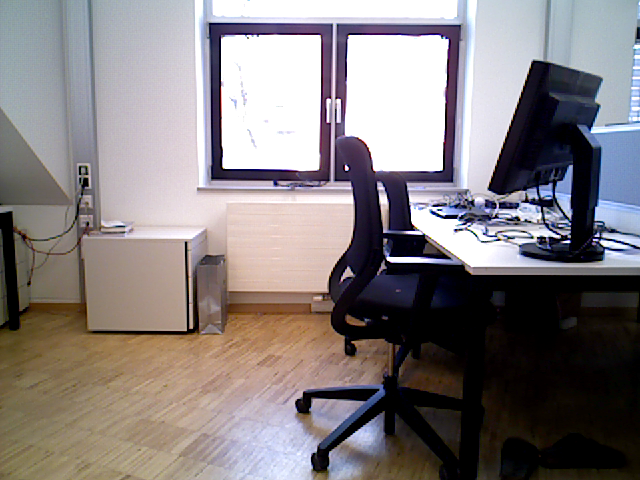
\includegraphics[width=0.4\textwidth, clip]{figures/peek/explore_lab_1bag1221.png}} &
\subfloat[dining room: 0.3918 \newline livingroom: 0.3093 \newline closet: 0.0878]{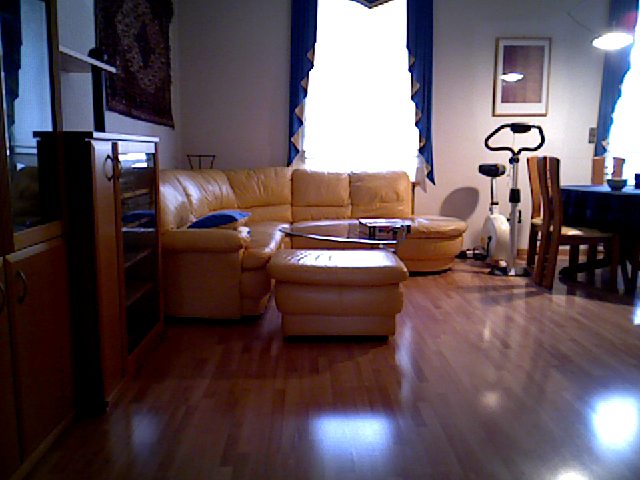
\includegraphics[width=0.4\textwidth, clip]{figures/peek/h5ebag117.png}} \\
\subfloat[kitchen: 0.4841 \newline restaurant kitchen: 0.2690 \newline kitchenette: 0.0439]{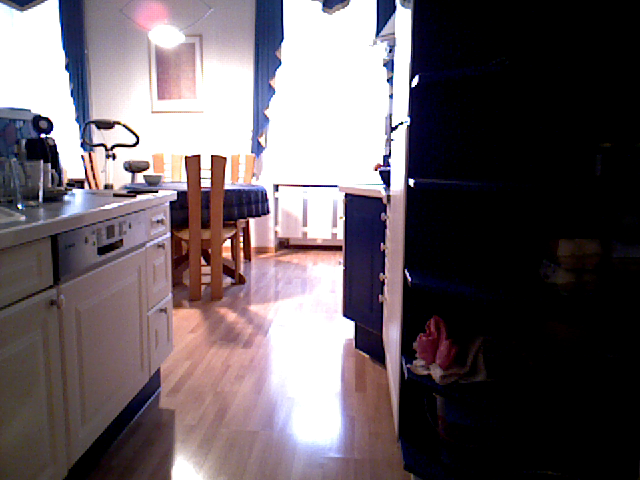
\includegraphics[width=0.4\textwidth, clip]{figures/peek/h7ebag41.png}} &
\subfloat[kitchen: 0.3211 \newline dining room: 0.2779 \newline restaurant kitchen: 0.0978]{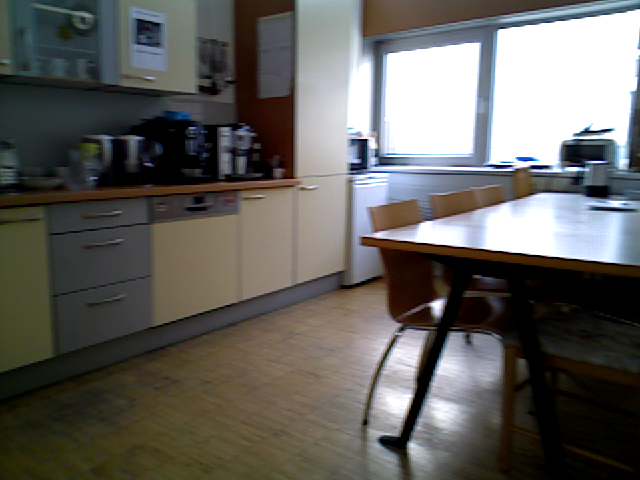
\includegraphics[width=0.4\textwidth, clip]{figures/peek/IST_explore_subag470.png}} \\
\subfloat[shower: 0.7556 \newline locker room: 0.1701 \newline martial arts gym: 0.0038]{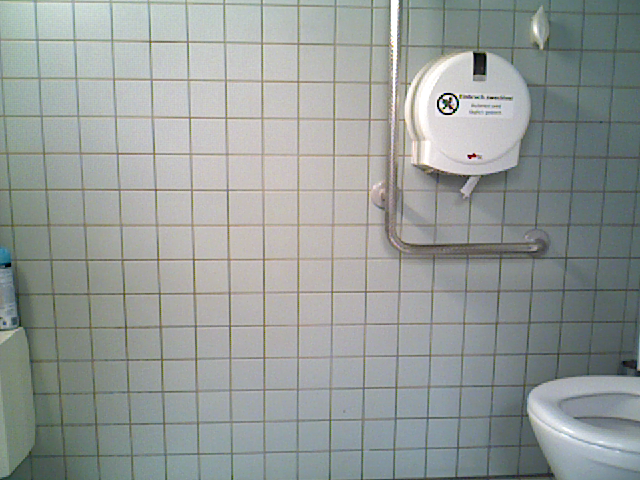
\includegraphics[width=0.4\textwidth, clip]{figures/peek/IST_explore_subag148.png}} &
\subfloat[classroom: 0.6971 \newline cafeteria: 0.0919 \newline conference center: 0.0256]{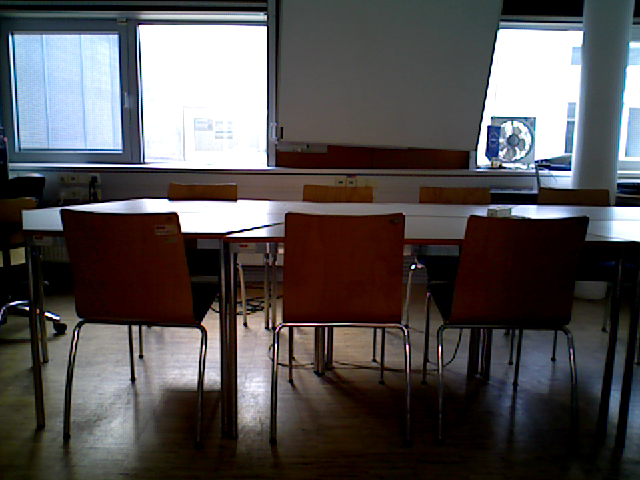
\includegraphics[width=0.4\textwidth, clip]{figures/peek/IST_explore_subag850.png}} 
\end{tabular}
\caption{Calculation of the frontiers: In those binary images black is 1 and white is 0; the gray accessible area in the last image is just for clarity}
\label{frontier_calc}
\end{figure}
\section{Search}


\begin{center}
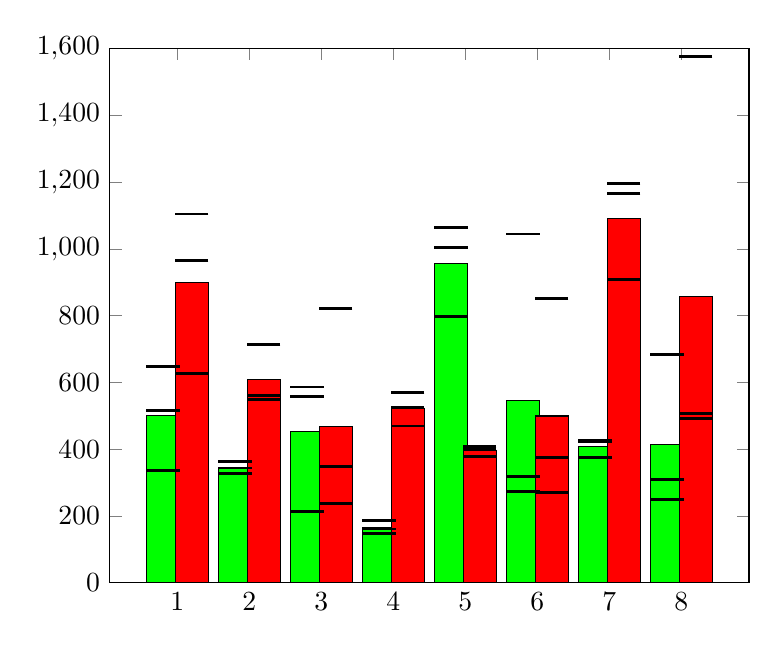
\begin{tikzpicture}
\centering
\begin{axis}[
xtick={1,2,3,4,5,6,7,8},
ymin=0, ymax=1600,
width=0.8\textwidth,
bar width=12pt,
scatter/classes={
a={mark=-,black,line width=1pt,mark size=6pt},%
b={mark=-,black,line width=1pt,mark size=6pt}}]%
\addplot[scatter,only marks, scatter src=explicit symbolic]
coordinates {
    (0.8, 516.495254517)[a]
    (0.8, 336.533113003)[a]
    (0.8, 647.728137016)[a]
    (1.8, 363.419975042)[a]
    (1.8, 343.370894432)[a]
    (1.8, 326.228244305)[a]
    (2.8, 586.39697957)[a]
    (2.8, 557.669190645)[a]
    (2.8, 214.022490501)[a]
    (3.8, 160.917860985)[a]
    (3.8, 187.370641708)[a]
    (3.8, 147.564922333)[a]
    (4.8, 1064.04291821)[a]
    (4.8, 1005.03980589)[a]
    (4.8, 797.52255702)[a]
    (5.8, 272.776754856)[a]
    (5.8, 318.844054461)[a]
    (5.8, 1044.20853162)[a]
    (6.8, 425.651885033)[a]
    (6.8, 375.731173277)[a]
    (6.8, 421.198181391)[a]
    (7.8, 249.180204391)[a]
    (7.8, 309.314040422)[a]
    (7.8, 684.093839407)[a]
    (1.2, 625.824002028)[b]
    (1.2, 1104.07050705)[b]
    (1.2, 965.284539938)[b]
    (2.2, 560.430487633)[b]
    (2.2, 714.455590963)[b]
    (2.2, 549.300167322)[b]
    (3.2, 237.52876091)[b]
    (3.2, 347.940049648)[b]
    (3.2, 822.017215014)[b]
    (4.2, 469.709306717)[b]
    (4.2, 526.516577721)[b]
    (4.2, 570.25410533)[b]
    (5.2, 377.531872988)[b]
    (5.2, 401.248581171)[b]
    (5.2, 407.269691706)[b]
    (6.2, 375.380629778)[b]
    (6.2, 270.339924097)[b]
    (6.2, 852.066253185)[b]
    (7.2, 907.174832344)[b]
    (7.2, 1195.6233592)[b]
    (7.2, 1166.11824775)[b]
    (8.2, 507.140073061)[b]
    (8.2, 1575.40179873)[b]
    (8.2, 490.799696922)[b]
};
\addplot[ybar,fill=green] coordinates {
    (0.8, 500.252168179)
    (1.8, 344.339704593)
    (2.8, 452.696220239)
    (3.8, 165.284475009)
    (4.8, 955.535093707)
    (5.8, 545.276446979)
    (6.8, 407.5270799)
    (7.8, 414.196028073)
    };
\addplot[ybar,fill=red] coordinates {
    (1.2, 898.393016339)
    (2.2, 608.062081973)
    (3.2, 469.162008524)
    (4.2, 522.159996589)
    (5.2, 395.350048622)
    (6.2, 499.26226902)
    (7.2, 1089.6388131)
    (8.2, 857.780522904)
    };
\end{axis}
\end{tikzpicture}
\end{center}


\begin{center}
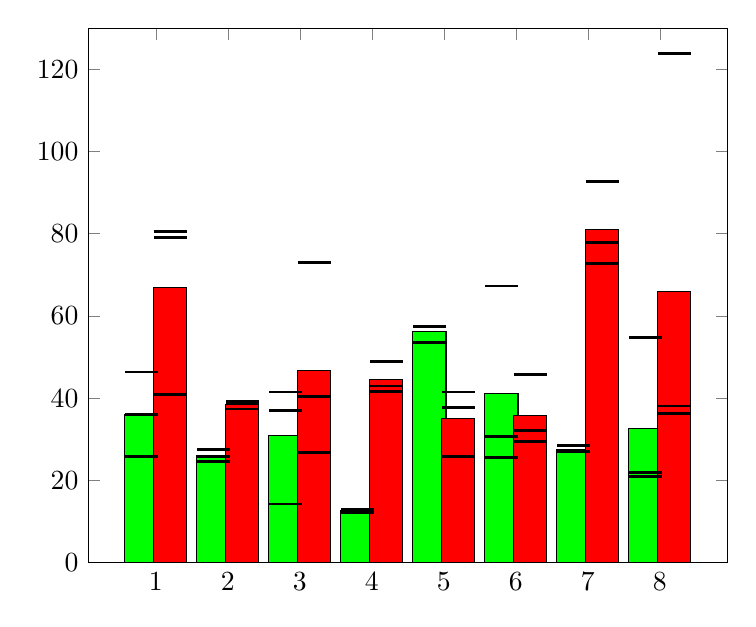
\begin{tikzpicture}
\centering
\begin{axis}[
xtick={1,2,3,4,5,6,7,8},
ymin=0, ymax=130,
width=0.8\textwidth,
bar width=12pt,
scatter/classes={
a={mark=-,black,line width=1pt,mark size=6pt},%
b={mark=-,black,line width=1pt,mark size=6pt}}]%
\addplot[scatter,only marks, scatter src=explicit symbolic]
coordinates {
    (0.8, 36.0462990646)[a]
    (0.8, 25.8572677796)[a]
    (0.8, 46.3369659858)[a]
    (1.8, 27.5183771793)[a]
    (1.8, 24.5872973823)[a]
    (1.8, 25.6953694644)[a]
    (2.8, 41.4675332412)[a]
    (2.8, 36.9404929352)[a]
    (2.8, 14.2131096213)[a]
    (3.8, 13.040464752)[a]
    (3.8, 12.58182994)[a]
    (3.8, 12.0977915009)[a]
    (4.8, 57.4493553078)[a]
    (4.8, 57.3581313606)[a]
    (4.8, 53.6199090129)[a]
    (5.8, 25.5068880058)[a]
    (5.8, 30.6138860794)[a]
    (5.8, 67.2832363072)[a]
    (6.8, 26.9133916064)[a]
    (6.8, 27.0155457101)[a]
    (6.8, 28.4238806649)[a]
    (7.8, 21.0112640972)[a]
    (7.8, 21.8385310971)[a]
    (7.8, 54.6950444656)[a]
    (1.2, 40.8781241112)[b]
    (1.2, 80.5366968831)[b]
    (1.2, 79.1306245474)[b]
    (2.2, 37.3345921959)[b]
    (2.2, 39.2489845791)[b]
    (2.2, 38.9003483464)[b]
    (3.2, 26.701472545)[b]
    (3.2, 40.309551522)[b]
    (3.2, 73.0273204978)[b]
    (4.2, 41.5151499647)[b]
    (4.2, 42.9570909759)[b]
    (4.2, 48.9559413629)[b]
    (5.2, 41.4574407677)[b]
    (5.2, 37.6911393151)[b]
    (5.2, 25.7423691633)[b]
    (6.2, 29.4670281238)[b]
    (6.2, 32.0744035115)[b]
    (6.2, 45.7013694978)[b]
    (7.2, 72.6905881441)[b]
    (7.2, 92.6424107254)[b]
    (7.2, 77.7918243583)[b]
    (8.2, 38.0714534023)[b]
    (8.2, 123.801759514)[b]
    (8.2, 36.1845726206)[b]
};
\addplot[ybar,fill=green] coordinates {
    (0.8, 36.08017761)
    (1.8, 25.933681342)
    (2.8, 30.8737119326)
    (3.8, 12.5733620643)
    (4.8, 56.1424652271)
    (5.8, 41.1346701308)
    (6.8, 27.4509393271)
    (7.8, 32.5149465533)
    };
\addplot[ybar,fill=red] coordinates {
    (1.2, 66.8484818472)
    (2.2, 38.4946417071)
    (3.2, 46.6794481883)
    (4.2, 44.4760607678)
    (5.2, 34.9636497487)
    (6.2, 35.7476003777)
    (7.2, 81.0416077426)
    (8.2, 66.0192618456)
    };
\end{axis}
\end{tikzpicture}
\end{center}


